\documentclass[10pt,a4paper]{article}
\usepackage[margin=1.75cm]{geometry}
\usepackage{booktabs}
\usepackage{graphicx}
\usepackage{caption}
\usepackage{float}
\usepackage{microtype}
\graphicspath{{figures/}}
\captionsetup{font=small,labelfont=bf}
\setlength{\parindent}{0pt}
\setlength{\parskip}{0.42em}
\renewcommand{\arraystretch}{1.12}

\title{\vspace{-1.2cm}\textbf{Attention-Based Segmentation from Stable Diffusion 1.5}\\[0.25em]
\large Ablations, interpretation, and cross-dataset generalization}
\author{}
\date{October 2026}

\begin{document}
\maketitle
\vspace{-1.5em}

\section{Experimental protocol}

Each released prompt and seed is regenerated for 30 inference steps.  Maps are
scored against the released mask and then discarded.  mIoU is the 20-class
macro average of pooled foreground IoU.  OVAM is reproduced with its released
dataset-specific thresholds and DenseCRF; token optimization is excluded.

Our revised final configuration retains all 16 CA layers.  Frozen CA head
filtering is applied to layers 0, 2, 5, 6, 7, 9, 10, 11, 12, 13, 14, and 15;
layers 1, 3, 4, and 8 use their all-head means.  CA is aggregated over calls
0--30.  The final $64\times64$ decoder SA module (U3.2) is applied once using
selected SA heads $\{0,1,2,4,5,6\}$ and calls 15--30.  Cross-attention attribution follows the
OVAM-compatible single-token convention.  The output uses percentile 1--99
normalization, threshold 0.45, and removal of connected components below 1\%
of the image.

\section{Cross-attention ablations}

\subsection{Denoising time}

\textit{Fixed configuration:} CA only on all 490 VOC-Sim images; all 15
non-middle CA modules at $16$, $32$, and $64$ resolution; all eight heads and
all class-token pieces; conditional CFG branch; OVAM max-after-resize
normalization; threshold 0.40; no SA fusion, DenseCRF, or component cleanup.
Only the included denoising calls change.

\begin{figure}[H]
  \centering
  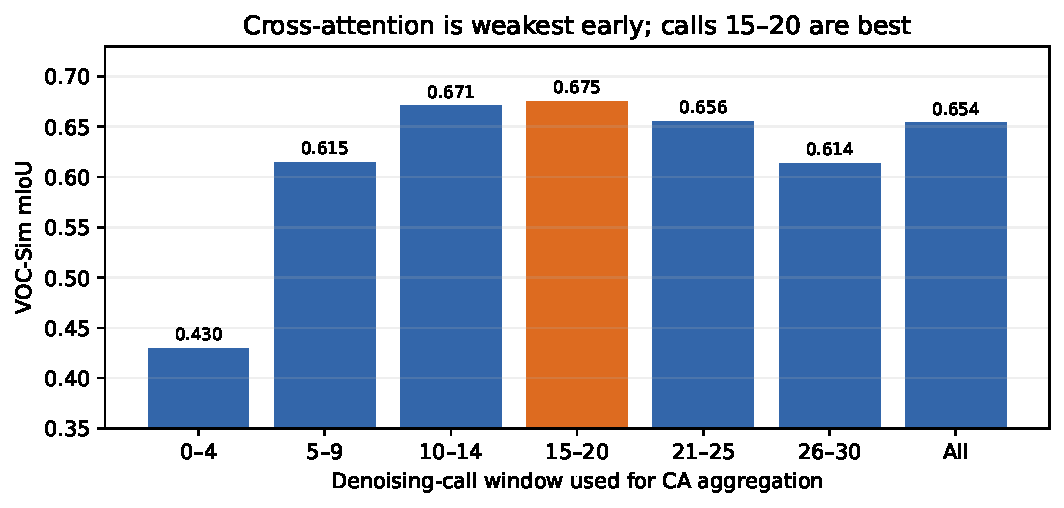
\includegraphics[width=0.82\linewidth]{ca_time_windows.pdf}
  \caption{CA-only time-window ablation on all 490 VOC-Sim images.  Very early
  calls are poorly localized; calls 15--20 are strongest in this aggregation.}
\end{figure}

\begin{table}[H]\centering\small
\begin{tabular}{lrrrrrrr}
\toprule
CA calls & 0--4 & 5--9 & 10--14 & 15--20 & 21--25 & 26--30 & All \\
\midrule
mIoU & 0.430 & 0.615 & 0.671 & \textbf{0.675} & 0.656 & 0.614 & 0.654 \\
\bottomrule
\end{tabular}
\caption{CA time-window mIoU under the fixed configuration above.}
\end{table}

\subsection{Resolution}

\textit{Fixed configuration:} CA only on all 490 VOC-Sim images; all denoising
calls 0--30; every CA module at the listed resolutions; all eight heads and all
class-token pieces; conditional CFG branch; OVAM max-after-resize
normalization; threshold 0.40; no SA fusion, DenseCRF, or component cleanup.
Only the retained resolutions change.

\begin{figure}[H]
  \centering
  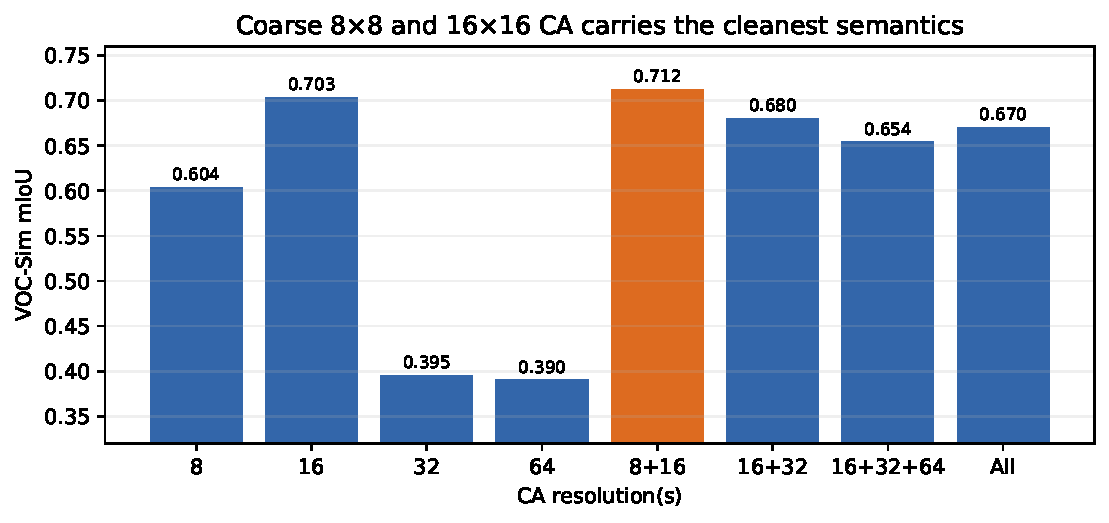
\includegraphics[width=0.86\linewidth]{ca_resolution.pdf}
  \caption{CA-only resolution screening.  Combining $8\times8$ and
  $16\times16$ maps is best in isolation.  The end-to-end revised system
  retains all layers and therefore all four resolutions.}
\end{figure}

\begin{table}[H]\centering\small
\begin{tabular}{lrrrrrrrr}
\toprule
CA resolution & 8 & 16 & 32 & 64 & 8+16 & 16+32 & 16+32+64 & All \\
\midrule
mIoU & 0.604 & 0.703 & 0.395 & 0.390 & \textbf{0.712} & 0.680 & 0.654 & 0.670 \\
\bottomrule
\end{tabular}
\caption{CA resolution mIoU under the fixed configuration above.}
\end{table}

Coarse $8\times8$ and $16\times16$ CA carries cleaner semantics in isolation.
The transfer experiment shows that discarding the other resolutions together
with their layers does not improve the final system.

\subsection{Individual layers}

\textit{Fixed configuration:} CA only on all 490 VOC-Sim images; one listed
module at a time; all denoising calls 0--30; all eight heads and all class-token
pieces; conditional CFG branch; percentile 1--99 normalization and threshold
0.45; no SA fusion or component cleanup.  This diagnostic averages image IoU,
so its values should be used to rank modules rather than compared numerically
with the class-macro mIoU tables.

\begin{figure}[H]
  \centering
  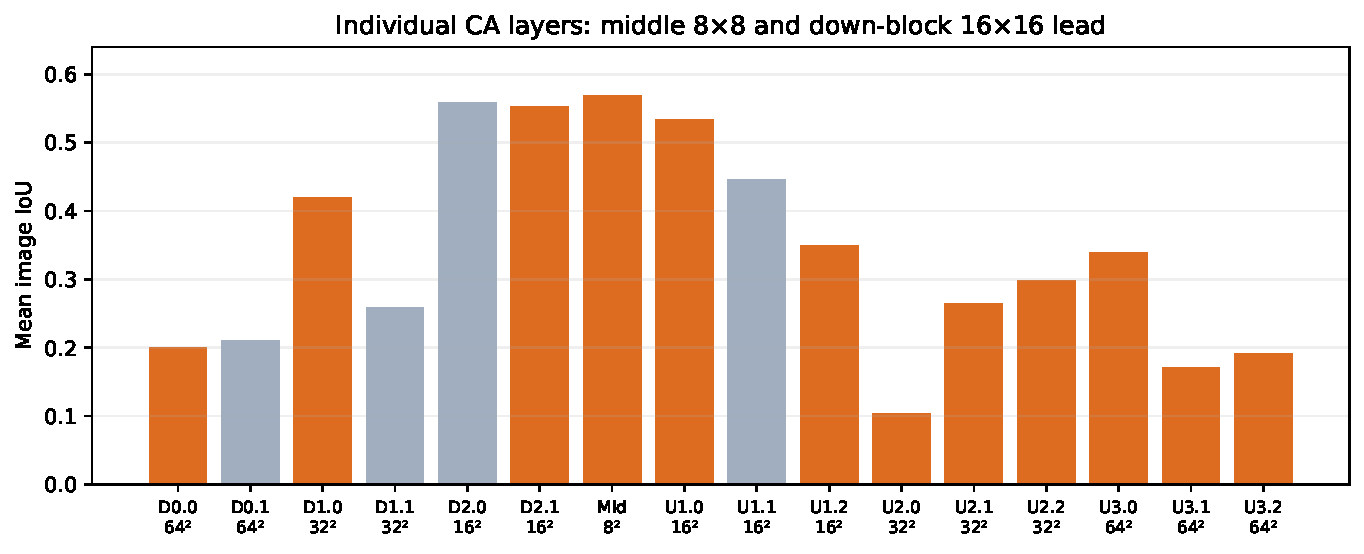
\includegraphics[width=0.98\linewidth]{ca_layers.pdf}
  \caption{Mean image IoU for individual CA modules.  Individual quality
  varies substantially, with the middle $8\times8$ block strongest.}
\end{figure}

\begin{table}[H]\centering\scriptsize
\begin{tabular}{crr@{\qquad}crr}
\toprule
Layer & Res. & Mean image IoU & Layer & Res. & Mean image IoU \\
\midrule
D0.0 & 64 & 0.200 & U1.1 & 16 & 0.446 \\
D0.1 & 64 & 0.211 & U1.2 & 16 & 0.350 \\
D1.0 & 32 & 0.420 & U2.0 & 32 & 0.104 \\
D1.1 & 32 & 0.258 & U2.1 & 32 & 0.264 \\
D2.0 & 16 & 0.559 & U2.2 & 32 & 0.299 \\
D2.1 & 16 & 0.552 & U3.0 & 64 & 0.340 \\
Mid  & 8  & \textbf{0.569} & U3.1 & 64 & 0.171 \\
U1.0 & 16 & 0.534 & U3.2 & 64 & 0.192 \\
\bottomrule
\end{tabular}
\caption{Individual CA-module screening; every listed module is retained by
the final system.}
\end{table}

The middle $8\times8$ block is strongest individually.  Individual rank is
not sufficient for layer removal: the earlier filtering removed both strong
and weak layers and reduced transfer performance.

\subsection{What CA head filtering contributes}

\textit{Fixed configuration:} all 16 CA layers and CA calls 0--30.  The
filtered seed uses frozen top-four head rankings for layers
$\{0,2,5,6,7,9,10,11,12,13,14,15\}$ and all-head means for layers
$\{1,3,4,8\}$; the control uses all eight heads everywhere.
Both use percentile 1--99 normalization.  ``After matched SA'' uses one pass
through U3.2 at $64\times64$, SA calls 15--30, SA heads
$\{0,1,2,4,5,6\}$, threshold 0.45, and 1\% component cleanup.

\begin{figure}[H]
  \centering
  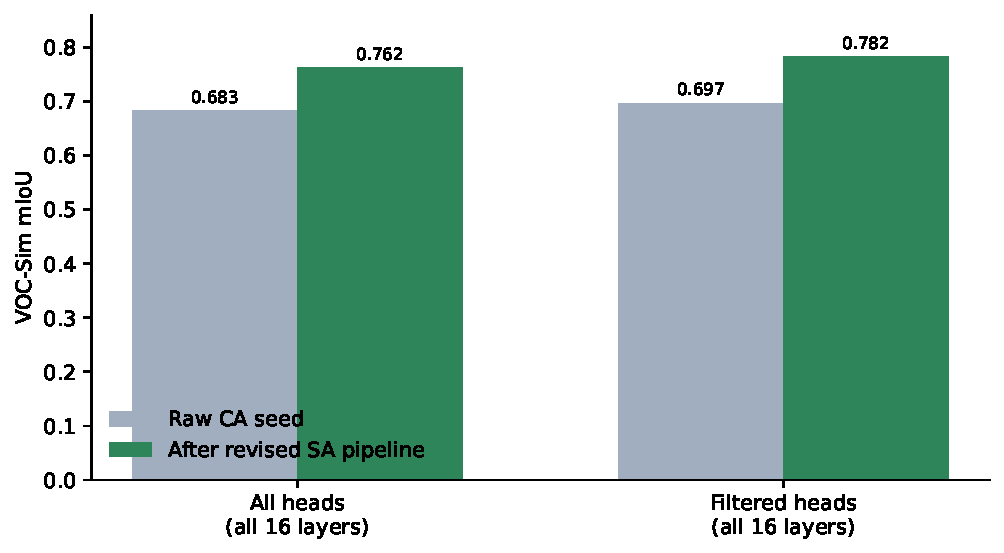
\includegraphics[width=0.78\linewidth]{ca_seed_sa_interaction.pdf}
  \caption{Both seeds retain all 16 CA layers.  Head filtering improves the
  raw seed and its output after the revised one-pass SA pipeline.}
\end{figure}

\begin{table}[H]\centering
\begin{tabular}{lrrr}
\toprule
CA seed & Raw mIoU & After matched SA & SA gain \\
\midrule
All 16 layers/all heads & 0.6830 & 0.7625 & +0.0795 \\
All 16 layers/filtered heads & \textbf{0.6969} & \textbf{0.7824} & +0.0855 \\
\bottomrule
\end{tabular}
\caption{Matched CA-head comparison for the revised all-layer system.}
\end{table}

Restoring all layers improves cross-dataset transfer.  Within that all-layer
system, CA head filtering contributes 0.0199 mIoU on VOC-Sim and 0.0069 on
COCO-Cap after the complete pipeline.

\section{Self-attention ablations}

\subsection{Which SA module?}

\textit{Fixed configuration:} all 490 VOC-Sim images; a CA seed formed from
the frozen top-four heads of CA layers
$\{0,2,5,6,7,9,10,11,12,13,14,15\}$, aggregated over CA calls 0--30 and
normalized by percentiles 1--99; all eight SA heads; SA calls
15--30; four propagation passes; percentile 1--99 output normalization;
threshold 0.45; no component cleanup.  Only the SA module changes.  As in the
layer diagnostic, the reported score is mean image IoU.

\begin{figure}[H]
  \centering
  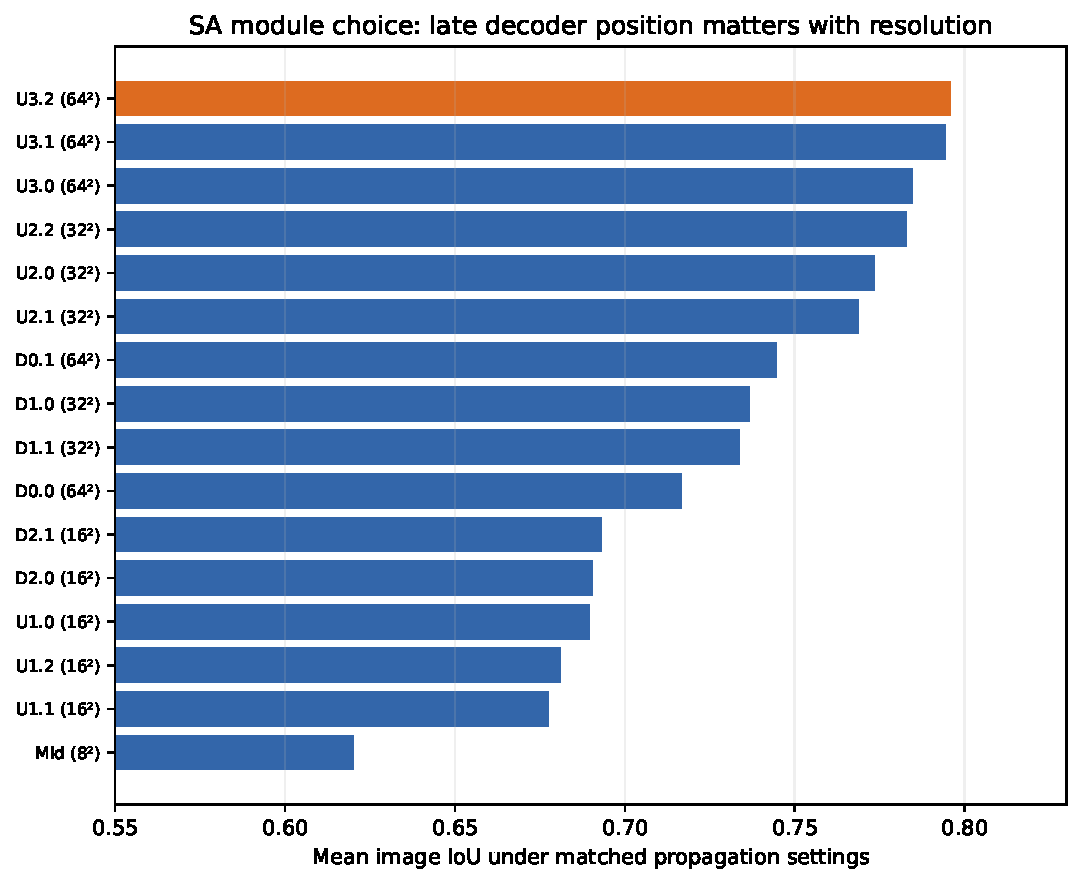
\includegraphics[width=0.78\linewidth]{sa_modules.pdf}
  \caption{Mean image IoU for every SA module under the fixed configuration
  above.  The final $64\times64$ upsampling module is best.}
\end{figure}

\begin{table}[H]\centering\scriptsize
\begin{tabular}{lrr@{\qquad}lrr}
\toprule
SA module & Res. & Mean image IoU & SA module & Res. & Mean image IoU \\
\midrule
D0.0 & 64 & 0.717 & U1.1 & 16 & 0.677 \\
D0.1 & 64 & 0.745 & U1.2 & 16 & 0.681 \\
D1.0 & 32 & 0.737 & U2.0 & 32 & 0.773 \\
D1.1 & 32 & 0.734 & U2.1 & 32 & 0.769 \\
D2.0 & 16 & 0.691 & U2.2 & 32 & 0.783 \\
D2.1 & 16 & 0.693 & U3.0 & 64 & 0.785 \\
Mid  & 8  & 0.620 & U3.1 & 64 & 0.794 \\
U1.0 & 16 & 0.689 & U3.2 & 64 & \textbf{0.796} \\
\bottomrule
\end{tabular}
\caption{SA-module screening under matched settings.}
\end{table}

The last $64\times64$ decoder module is best.  Both decoder position and
resolution matter; the early $64\times64$ modules are much weaker.

\subsection{Which denoising calls?}

\textit{Fixed configuration:} all 16 CA layers and CA calls 0--30; frozen CA
head filtering; one pass through U3.2 at $64\times64$; SA heads
$\{0,1,2,4,5,6\}$; percentile 1--99 normalization; threshold 0.45; and 1\%
component cleanup.  Only the SA call set changes.  The same frozen
configuration is evaluated on all 490 VOC-Sim and 707 COCO-Cap images.

\begin{figure}[H]
  \centering
  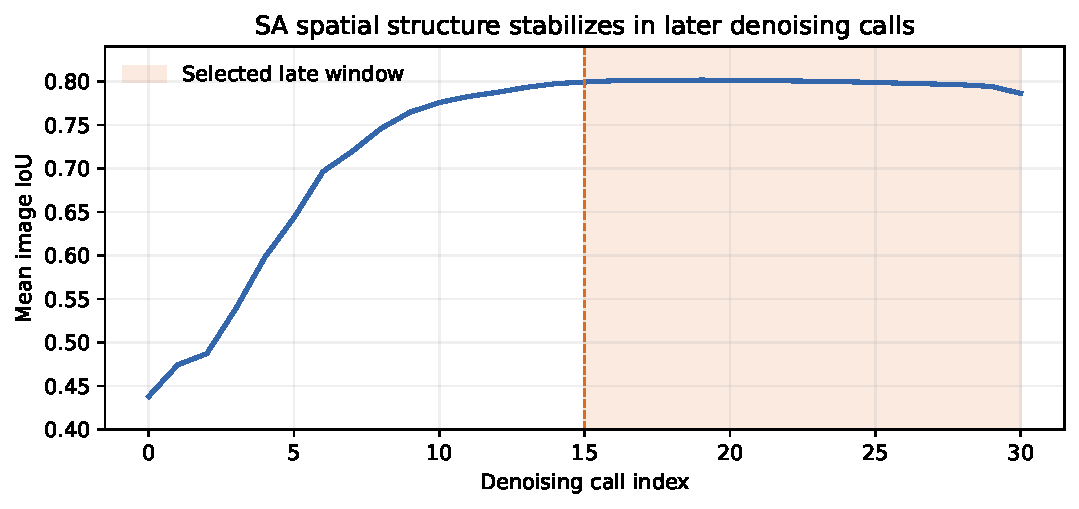
\includegraphics[width=0.80\linewidth]{sa_timesteps.pdf}
  \caption{Matched timestep-window screening in the selected-SA-head
  predecessor.  Calls 15--30 improve both datasets.}
\end{figure}

\begin{table}[H]\centering\small
\begin{tabular}{lrrr}
\toprule
Dataset & Calls 15--30 & All calls & Late-window gain \\
\midrule
VOC-Sim & \textbf{0.7824} & 0.7802 & +0.0022 \\
COCO-Cap & \textbf{0.6322} & 0.6240 & +0.0083 \\
\bottomrule
\end{tabular}
\caption{Leave-one-change comparison for SA timestep filtering.}
\end{table}

Late calls provide a small VOC improvement and a clearer COCO-Cap improvement.
The final system therefore retains calls 15--30.

\subsection{Which SA heads?}

\textit{Fixed configuration:} all 16 CA layers and CA calls 0--30; frozen CA
head filtering; one pass through U3.2 at $64\times64$; SA calls 15--30;
percentile 1--99 normalization; threshold 0.45; and 1\% component cleanup.
Only the SA head set changes.  ``Selected'' means
$\{0,1,2,4,5,6\}$; ``all'' means heads 0--7.

\begin{table}[H]\centering\small
\begin{tabular}{lrrr}
\toprule
Dataset & Selected heads & All heads & Selected-head gain \\
\midrule
VOC-Sim & 0.7824 & \textbf{0.7837} & -0.0013 \\
COCO-Cap & \textbf{0.6322} & 0.6274 & +0.0049 \\
\bottomrule
\end{tabular}
\caption{Leave-one-change comparison of the SA-head sets on both datasets.}
\end{table}

All SA heads improve VOC-Sim by 0.0013 mIoU, but selected heads improve the
untuned COCO-Cap result by 0.0049.  The final system retains the selected set.

\section{What changes in the final mask?}

\begin{table}[H]\centering
\begin{tabular}{lrrr}
\toprule
Measure & Implemented OVAM & Final method & Change \\
\midrule
Foreground precision & 0.710 & 0.866 & +0.156 \\
Foreground recall & 0.895 & 0.876 & $-0.019$ \\
Predicted foreground area & 0.467 & 0.375 & $-0.092$ \\
Ground-truth foreground area & 0.370 & 0.370 & --- \\
\bottomrule
\end{tabular}
\caption{Binary-mask diagnostics for the revised final system over 490
VOC-Sim images.}
\end{table}

Precision rises from 0.710 to 0.866 while recall changes from 0.895 to 0.876.
The revised mask nearly matches the true foreground area, showing that the
gain mainly comes from suppressing false foreground.

\begin{table}[H]\centering\small
\begin{tabular}{lrl}
\toprule
Class-area quartile & Mean gain & Classes \\
\midrule
Q1 (smallest) & +0.0969 & bird, aeroplane, bottle, chair, boat \\
Q2 & +0.0919 & table, train, bicycle, car, bus \\
Q3 & +0.0747 & motorbike, horse, dog, cow, person \\
Q4 (largest) & +0.0662 & sheep, sofa, plant, tv, cat \\
\bottomrule
\end{tabular}
\caption{Revised-system gain grouped by class-average foreground area.}
\end{table}

Every class-size quartile improves.  The declining trend indicates that OVAM
already handles many large foreground objects well, while the revised system
has more room to suppress false foreground around smaller objects.

\section{Generalization to COCO-Cap}

The final configuration uses all 16 CA layers, CA calls 0--30, frozen CA head
filtering, one U3.2 SA pass, SA calls 15--30, and selected SA heads
$\{0,1,2,4,5,6\}$.

\begin{table}[H]\centering
\begin{tabular}{llrrrr}
\toprule
Dataset & Method & Images & Classes & mIoU & Gain over OVAM \\
\midrule
VOC-Sim & Implemented OVAM & 490 & 20 & 0.6934 & --- \\
VOC-Sim & Final method & 490 & 20 & \textbf{0.7824} & \textbf{+0.0890} \\
\addlinespace
COCO-Cap & OVAM & 707 & 20 & 0.5719 & --- \\
COCO-Cap & Final method, frozen & 707 & 20 & \textbf{0.6322} & \textbf{+0.0603} \\
\bottomrule
\end{tabular}
\caption{Primary comparison.  VOC-Sim is the development dataset; COCO-Cap is
the untuned generalization dataset.}
\end{table}

The authors' released VOC-Sim masks score 0.7036.  We use our live 0.6934
implementation for the matched VOC-Sim comparison because both methods use the
same regenerated trajectories.

\end{document}
